\documentclass[16pt, spanish]{article}

\usepackage{array}
\usepackage[spanish]{babel}
\usepackage{anysize}
\usepackage{graphicx}
\usepackage{amsmath}
\usepackage{amsfonts}
\usepackage{multicol}
\usepackage{float}
\usepackage{multirow}
\usepackage{amssymb}
\usepackage{rmfbib}


\marginsize{2cm}{2cm}{1cm}{1cm}
\begin{document}

\title{{\textbf{ACTIVIDAD 2.7}}\\{\small Universidad de Guadalajara}\\}
\date{\small Noviembre de 2021}
\author{\small Varela Tavares Gabriel}
\maketitle

 

\section*{Consulta y cambios en procesos MAP y REDUCE}

Se arrancan los servicios de Hadoop y de Apache Hive. Se usa la base de datos anterior y luego \textbf{\textit{SELECT * FROM aseg2020 ORDER BY cve\_entidad LIMIT 100;}} Esto muestra MAP:4 y REDUCE:1.

\begin{center}
 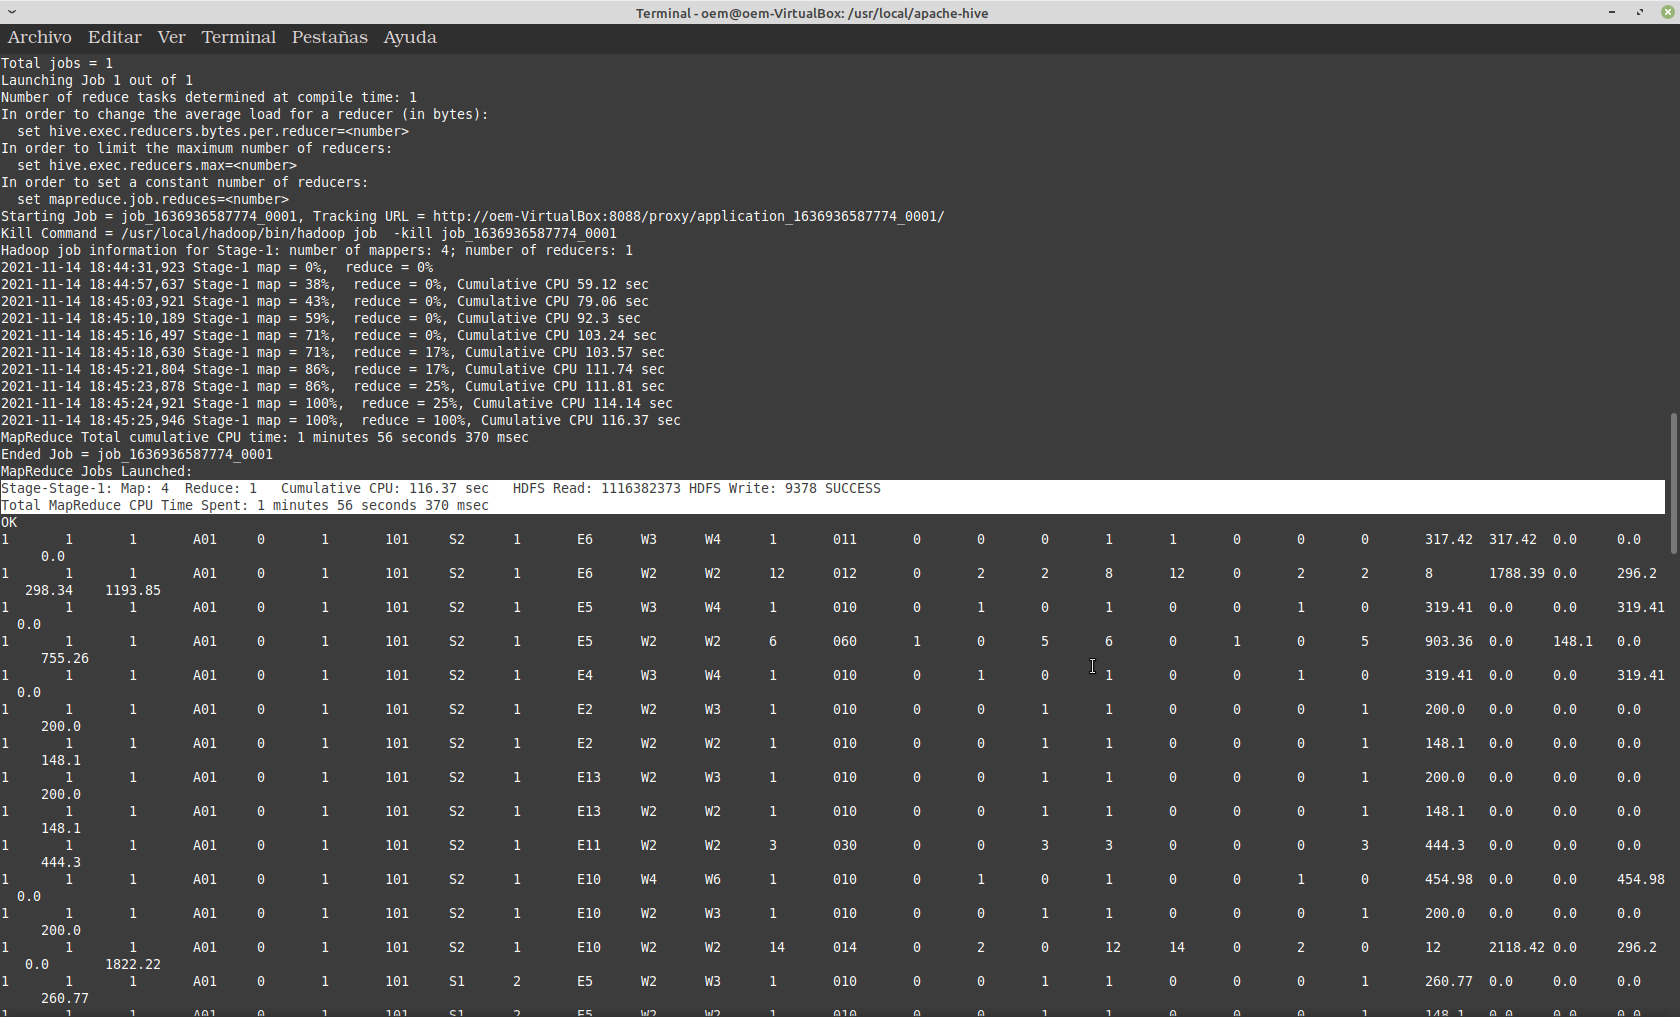
\includegraphics[width=0.9\columnwidth]{consulta.png}\\
 \footnotesize{}
\end{center}
\vspace{.5cm}

También se hizo la consulta con order by cve\_subdelegacion de la siguiente manera: \textbf{\textit{SELECT * FROM aseg2020 ORDER BY cve\_subdelegacion LIMIT 100;}}. Esta ejecución realiza MAP:4 y REDUCE:1.

\begin{center}
 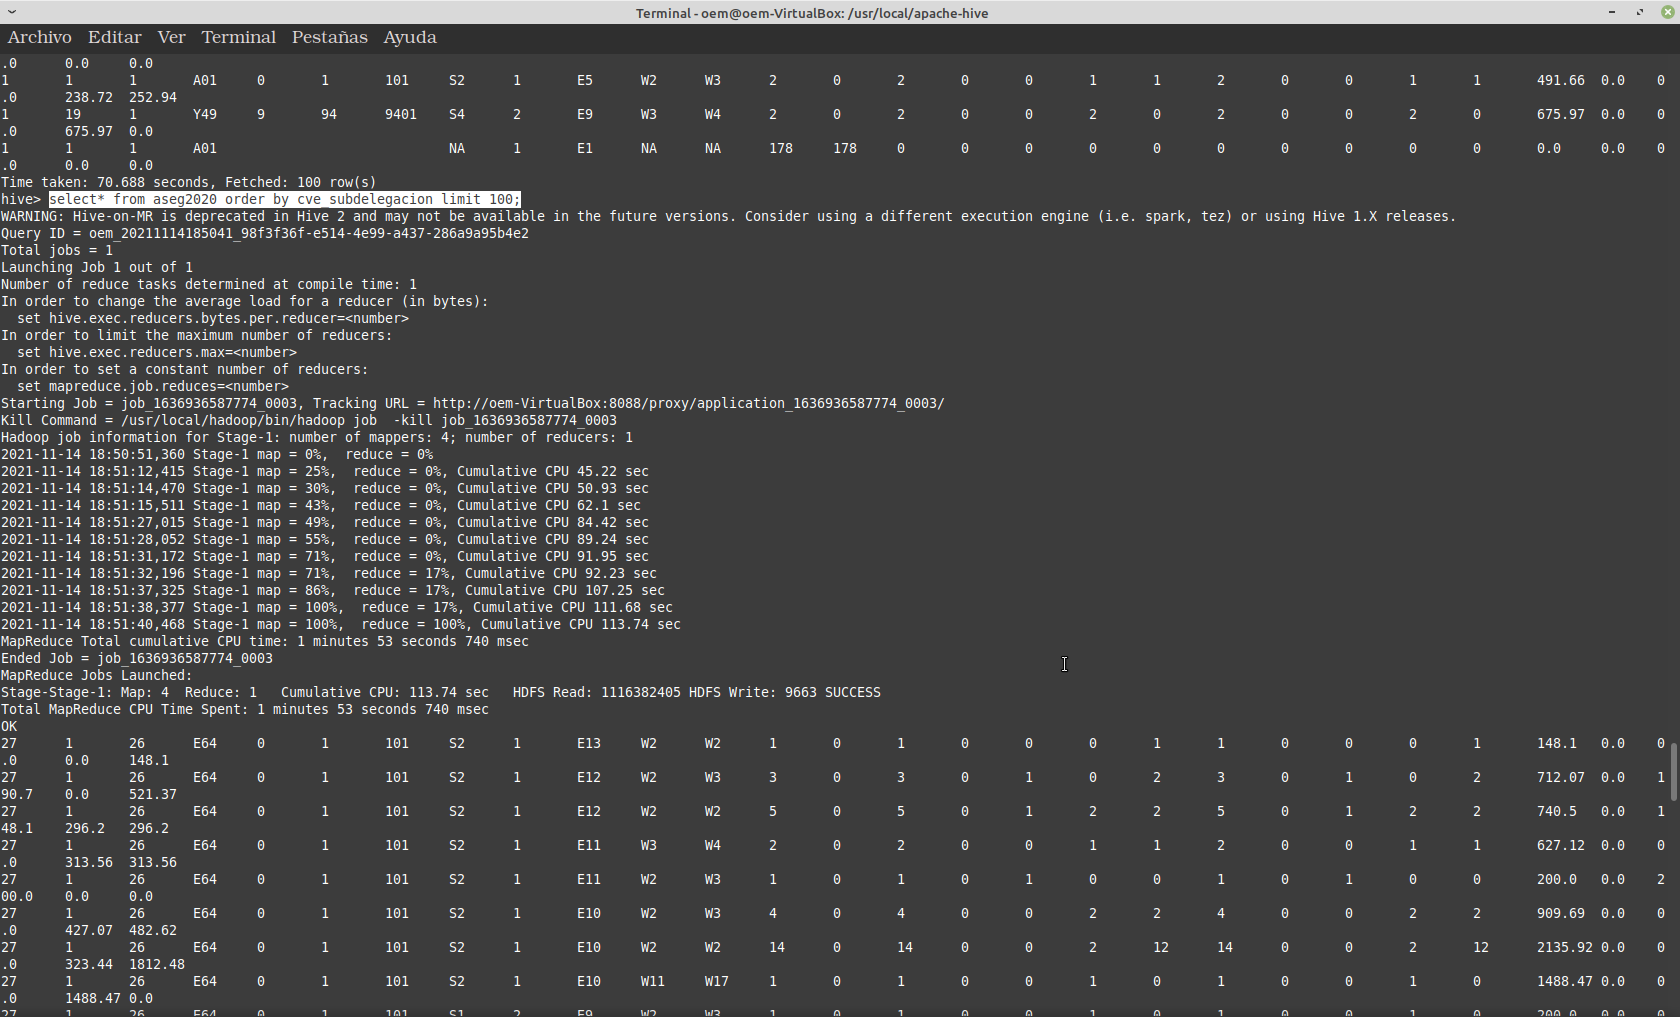
\includegraphics[width=0.9\columnwidth]{consulta2.png}\\
 \footnotesize{}
\end{center}
\vspace{.5cm}














\end{document}